\chapter{Project Integration Management}

Our first step in ensuring the successful delivery of this project to MYH is to gain a comprehensive understanding of their primary goals and objectives. This part provides an overview of the main objectives, initial proposals, and business case studies that have been developed in consultation with the MYH.

\section{Case Study}

Manage Your Health, Inc. (MYH) is a global healthcare provider ranked among the Fortune 500. With over 25,000 employees worldwide, including 20,000 full-time and 5,000 part-time workers, MYH is committed to cutting internal costs, enhancing cross-selling of products, and leveraging new web technologies to foster collaboration among employees, customers, and suppliers, thereby enhancing the delivery of healthcare products and services.

MYH has identified three potential projects in line with their strategic objectives:

\begin{enumerate}[label=\textbf{\arabic*.}]
    \item \textbf{Health Coverage Costs Business Model:} This project involves developing a secure application to model and analyze healthcare expenses. It requires an initial investment of \$100,000 and is projected to save \$20 annually for each full-time employee.
    
    \item \textbf{Web-Enhanced Communications System:} The goal of this project is to implement a web-based system that streamlines the development and delivery of products. With a development cost of \$3 million, the system is expected to save \$2 million annually, notwithstanding ongoing maintenance costs.
    
    \item \textbf{Recreation and Wellness Intranet Project:} This initiative aims to launch an intranet application to enhance employee health and wellness, potentially reducing healthcare premiums and saving \$30 per employee each year through better health outcomes.
\end{enumerate}

MYH requests a preliminary analysis to determine which project best meets their strategic goals and asks for a detailed business plan for the chosen proposal.

\section{Project Analysis}

In response to the request from MYH, we initiated a preliminary analysis of the proposed projects. 

\subsection{Objectives Analysis}

The analysis began with an understanding of the strategic goals of MYH. These objectives were elucidated through comprehensive discussions with MYH's visionary leaders. The key strategic goals derived from these discussions are summarized in Table \ref{tab:myh_goals}.

\begin{table}[h]
    \centering
    \begin{tabular}{|c|p{10cm}|}
    \hline
    \textbf{Goal} & \textbf{Description} \\
    \hline
    Reduce-Cost & Aim to decrease internal costs to enhance efficiency and boost profitability. \\
    \hline
    Business-Growth & Increase market penetration and revenue through enhanced cross-selling opportunities. \\
    \hline
    Develop & Improve collaboration among employees, customers, and suppliers with new web-based technologies, thereby optimizing the development and delivery of healthcare products and services. \\
    \hline
    \end{tabular}
    \caption{Strategic Goals of Manage Your Health, Inc.}
    \label{tab:myh_goals}
\end{table}

\FloatBarrier

This structured approach allows us to align each project proposal with MYH's strategic objectives, facilitating an informed decision-making process for developing the subsequent business plan.

\subsection{Proposal Analysis}

Once the objectives were established, our team conducted a comprehensive analysis of each proposal to ensure they aligned with MYH's goals. We focused on several key metrics, assigning different weights to each criterion based on its importance:

\begin{itemize}
    \item Tie to business strategy - 10\%
    \item Upfront cost - 25\%
    \item Potential net savings - 25\%
    \item Realistic technology - 15\%
    \item In-house expertise - 10\%
    \item Potential resistance - 15\%
\end{itemize}

The findings of our analysis are summarized in Table \ref{tab:project_com}, providing a clear comparison of how each proposal measures up against the set criteria.

\begin{table}[h]
    \centering
    \caption{Comparison of Project Criteria and Their Impact}
    \label{tab:project_com}
    \begin{tabularx}{\textwidth}{>{\hsize=0.7\hsize}X>{\hsize=0.5\hsize}X>{\hsize=1.2\hsize}X>{\hsize=1.3\hsize}X>{\hsize=1.3\hsize}X}
    \toprule
    \textbf{Criteria} & \textbf{Weight} & \textbf{Health Coverage Costs Business Model} & \textbf{Web-Enhanced Communications System} & \textbf{Recreation and Wellness Intranet Project} \\
    \midrule
    Tie-to business strategy & 10\% & Reduce-Cost (1/3) & Business-Growth, Develop (2/3) & Reduce-Cost (1/3) \\
    Upfront cost & 25\% & \$100,000 & \$3,000,000 & \$200,000 \\
    Potential net savings & 25\% & \$1,600,000 & \$6,000,000 & \$2,400,000 \\
    Realistic technology & 15\% & Data Analysts needed to analyze the premiums of current and past employees linked to 10 different insurance companies. & The project is highly achievable with modern technology, as we all have experience with similar systems. & The project is highly achievable with modern technology, as we all have experience with similar systems. \\
    In-house expertise & 10\% & Organization might need to hire more experienced Data Analysts, even though we have expert developers to implement the application to analyze the data. & New components to be implemented and new services to be provided, such as delivery services, customer support, and suppliers management, necessitate hiring quite a few staff. & Project is easy to implement with proper guidance from a Team Lead. \\
    Potential resistance & 15\% & Project might not face much resistance since the application is relatively easy to build. & Project might not face much resistance since the application is relatively easy to build. & Senior employees might resist involvement in recreational programs due to greater responsibilities like family care. Other employees might also show disinterest. \\
    \bottomrule
    \end{tabularx}
\end{table}

\FloatBarrier

\subsection{Weighted Model} \label{sec:wm}

To further analyze our findings, we quantified the results from Table \ref{tab:project_com} to create a weighted model, as shown in Table \ref{tab:project_com_2}.

\begin{table}[h]
    \centering
    \begin{tabularx}{\textwidth}{>{\hsize=0.7\hsize}X>{\hsize=0.5\hsize}X>{\hsize=1.2\hsize}X>{\hsize=1.3\hsize}X>{\hsize=1.3\hsize}X}
    \toprule
    \textbf{Criteria} & \textbf{Weight} & \textbf{Health Coverage Costs Business Model} & \textbf{Web-Enhanced Communications System} & \textbf{Recreation and Wellness Intranet Project} \\
    \midrule
    Tie to business strategy & 10\% & 50 & 70 & 60 \\
    Upfront cost & 25\% & 70 & 35 & 85 \\
    Potential net savings & 25\% & 70 & 30 & 90 \\
    Realistic technology & 15\% & 60 & 85 & 75 \\
    In-house expertise & 10\% & 55 & 40 & 80 \\
    Potential resistance & 15\% & 80 & 85 & 60 \\
    \midrule
    \textbf{Total} & 100\% & 66.5 & 52.75 & 78 \\
    \bottomrule
    \end{tabularx}
    \caption{Comparison of Project Criteria and Their Impact (Weighted Model)}
    \label{tab:project_com_2}
\end{table}

\begin{figure}[ht]
    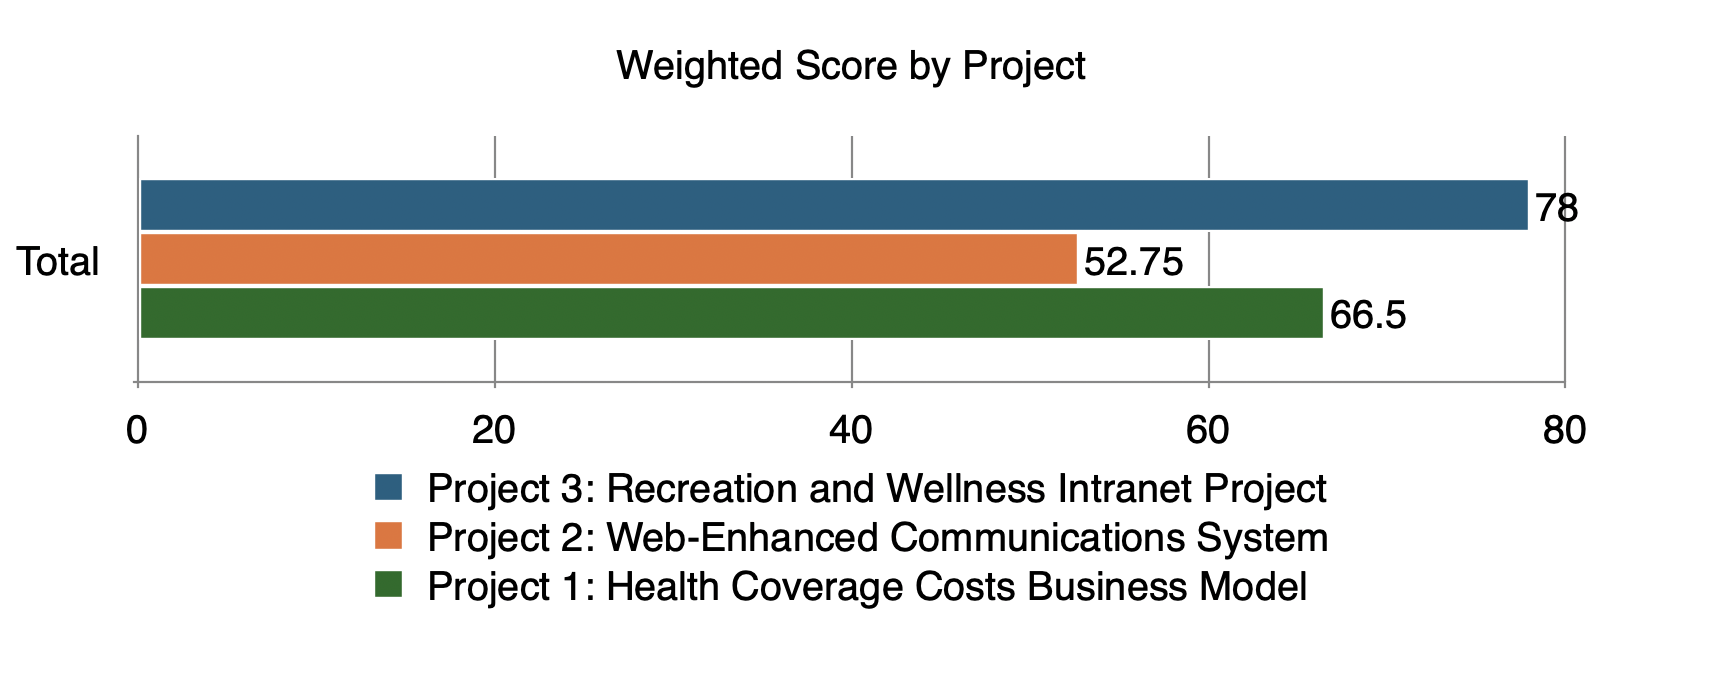
\includegraphics[width=\textwidth]{images/wsm.png}
    \caption{Weighted Score Model}
    \label{fig:wsm}
\end{figure}

The chart depicted in Figure \ref{fig:wsm} provides a visual representation of the evaluation model. From this chart, we can see that \textbf{Project 3: Recreation and Wellness Intranet Project} is the most preferred, followed by \textbf{Project 1: Health Coverage Costs Business Model}. This visual aids in understanding the relative preferences based on the weighted scoring of each project.

\subsection{Financial Analysis} \label{sec:fa}

To enhance our project selection process, we conducted a financial analysis to ensure that the chosen projects provide maximum benefit to MYH. Our team evaluated the Net Present Value (NPV) and Return on Investment (ROI) for each project to verify alignment with financial objectives and to ensure optimal returns. The detailed metrics and results of this analysis are summarized in the subsequent sections, providing a clear basis for our project recommendations.

\subsubsection*{Net Present Value (NPV)}
Net Present Value (NPV) is a financial metric used to evaluate the profitability of an investment or project. It represents the difference between the present value of cash inflows and the present value of cash outflows over the investment's lifetime. NPV is calculated using the formula:

\[
\text{NPV} = \sum_{t=0}^{n} \frac{C_t}{(1 + r)^t}
\]

where:
\begin{itemize}
    \item \( C_t \) represents the cash flow at time \( t \),
    \item \( r \) is the discount rate,
    \item \( t \) is the time period (usually in years),
    \item \( n \) is the total number of periods.
\end{itemize}

This formula discounts each of the cash flows back to their present value and then sums them up. A positive NPV indicates that the projected earnings exceed the anticipated costs, thus making it a potentially profitable investment.

\subsubsection*{Return on Investment (ROI)}
Return on Investment (ROI) is a financial metric used to measure the efficiency of an investment or to compare the efficiencies of several different investments. ROI measures the amount of return on an investment relative to the investment's cost, calculated as:

\[
\text{ROI} = \left(\frac{\text{Total Benefits} - \text{Total Costs}}{\text{Total Costs}}\right) \times 100\%
\]

where:
\begin{itemize}
    \item \(\text{Total Benefits}\) represents the total cash inflows from the investment,
    \item \(\text{Total Costs}\) represents the total cash outflows for the investment.
\end{itemize}

ROI is expressed as a percentage; a higher ROI means the investment gains compare favorably to its cost. It is used to evaluate the efficiency of an investment or compare the efficiencies of several different investments.

\subsubsection*{Financial Analysis of Projects}
The NPV and ROI calculations for the projects are detailed and summarized in Table \ref{tab:financial_analysis}. This table provides insights into the financial viability and potential profitability of each project, aiding in the decision-making process.

\begin{table}[ht]
    \centering
    \caption{Financial Analysis for Three Projects}
    \label{tab:financial_analysis}
    \begin{tabular}{lcccccc}
    \toprule
    \textbf{Item} & \textbf{Year 0} & \textbf{Year 1} & \textbf{Year 2} & \textbf{Year 3} & \textbf{Year 4} & \textbf{Total} \\
    \midrule
    \multicolumn{7}{c}{\textbf{Project 1: Health Coverage Costs Business Model}} \\
    \midrule
    Benefits & \$0 & \$400,000 & \$400,000 & \$400,000 & \$400,000 & \$1,600,000 \\
    Cost & \$100,000 & \$0 & \$0 & \$0 & \$0 & \$100,000 \\
    Cashflow & -\$100,000 & \$400,000 & \$400,000 & \$400,000 & \$400,000 & \$1,500,000 \\
    \textbf{NPV(D=8\%)} & \multicolumn{5}{c}{\textbf{\$1,134,121.05}} \\
    \textbf{ROI} & \multicolumn{5}{c}{\textbf{1500\%}} \\
    \midrule
    \multicolumn{7}{c}{\textbf{Project 2: Web-Enhanced Communications System}} \\
    \midrule
    Benefits & \$0 & \$2,000,000 & \$2,000,000 & \$2,000,000 & \$0 & \$6,000,000 \\
    Cost & \$3,000,000 & \$600,000 & \$600,000 & \$600,000 & \$600,000 & \$5,400,000 \\
    Cashflow & -\$3,000,000 & \$1,400,000 & \$1,400,000 & \$1,400,000 & -\$600,000 & \$600,000 \\
    \textbf{NPV(D=8\%)} & \multicolumn{5}{c}{\textbf{\$154,553.58}} \\
    \textbf{ROI} & \multicolumn{5}{c}{\textbf{11\%}} \\
    \midrule
    \multicolumn{7}{c}{\textbf{Project 3: Recreation and Wellness Intranet Project}} \\
    \midrule
    Benefits & \$0 & \$600,000 & \$600,000 & \$600,000 & \$600,000 & \$2,400,000 \\
    Cost & \$200,000  & \$0 & \$0 & \$0 & \$0 & \$200,000  \\
    Cashflow & -\$200,000  & \$600,000 & \$600,000 & \$600,000 & \$600,000 & \$2,200,000 \\
    \textbf{NPV(D=8\%)} & \multicolumn{5}{c}{\textbf{\$1,654,885.28}} \\
    \textbf{ROI} & \multicolumn{5}{c}{\textbf{1100\%}} \\
    \bottomrule
    \end{tabular}
\end{table}


\subsection{Project Selection}

After a thorough analysis of each project, considering both financial metrics (Section \ref{sec:fa}) and qualitative criteria (Section \ref{sec:wm}) we made a final decision on project selection for MYH.

\begin{itemize}
    \item \textbf{Project 1: Health Coverage Costs Business Model}
    \begin{itemize}
        \item \textbf{NPV}: \$1,134,121.05
        \item \textbf{ROI}: 1500\%
        \item \textbf{Decision}: Project 1 is appealing for selection due to its high ROI and substantial positive NPV, indicating significant profitability and efficient capital utilization but requires careful consideration of the additional staffing needs and its modest strategic tie.
    \end{itemize}

    \item \textbf{Project 2: Web-Enhanced Communications System}
    \begin{itemize}
        \item \textbf{NPV}: \$154,553.58
        \item \textbf{ROI}: 11\%
        \item \textbf{Decision}: Not recommended for immediate selection due to its lower ROI and marginal NPV, suggesting limited profitability and efficiency.
    \end{itemize}

    \item \textbf{Project 3: Recreation and Wellness Intranet Project}
    \begin{itemize}
        \item \textbf{NPV}: \$1,654,885.28
        \item \textbf{ROI}: 1100\%
        \item \textbf{Decision}: Project 3 offers a very high ROI and the highest NPV among the evaluated projects, ensuring excellent profitability and effective capital use. It presents a balanced option with moderate costs, significant expertise availability, and high feasibility with current technology, though it might face resistance impacting its implementation.
    \end{itemize}
\end{itemize}

Based on the comprehensive analysis of financial metrics along with the qualitative assessments, \textbf{Project 3: Recreation and Wellness Intranet Project} stands out as the optimal choice. This project not only demonstrates substantial financial returns but also aligns with technological feasibility and existing in-house expertise. Although there may be some resistance from senior employees, its moderate initial investment and significant long-term benefits warrant its selection. The project's strategic alignment with enhancing employee engagement and wellness further supports its potential for positive organizational impact.


\section{Business Case}
This section presents the business case for \textbf{Project 3: Recreation and Wellness Intranet Project}, proposed by Manage Your Health Inc. (MYH). 

The business case was developed based on the objectives, mission statement, goals, project phases, and financial and market analyses of the project. The results are summarized in Table \ref{tab:project_summary}. The detailed business case prepared by the project manager is presented below.


\begin{longtable}{|p{0.25\textwidth}|p{0.7\textwidth}|}
    \caption{Business case for Recreation and Wellness Intranet Project} \label{tab:project_summary} \\
    \hline
    \textbf{Section} & \textbf{Details} \\
    \hline
    \endfirsthead
    
    \multicolumn{2}{c}%
    {\tablename\ \thetable\ -- \textit{Continued from previous page}} \\
    \hline
    \textbf{Section} & \textbf{Details} \\
    \hline
    \endhead
    
    \hline
    \endfoot
    
    \hline
    \endlastfoot
    
    \textbf{Project Overview} & 
        \begin{itemize}
            \item \textbf{Project Manager:} Tony Prince
            \item \textbf{Client:} Manage Your Health Inc.
            \item \textbf{Duration:} 6 months
            \item \textbf{Budget:} \$200,000
        \end{itemize} \\
    \hline
    \textbf{Executive Summary} & 
        Aims to improve employee health and reduce healthcare costs by engaging employees in wellness and recreational programs, targeting savings of at least \$30 per employee per year. \\
    \hline
    \textbf{Mission Statement} & 
        To empower and engage employees in enhancing their health and well-being through accessible digital wellness solutions. \\
    \hline
    \textbf{Objectives} & 
        \begin{enumerate}
            \item Reduce healthcare costs by improving employee health.
            \item Enhance employee productivity and morale through structured wellness programs.
            \item Offer a tailored intranet solution to promote health management.
        \end{enumerate} \\
    \hline
    \textbf{Project Phases} & 
        Initiation, Planning, Execution, Monitoring and Control, Closure, and Post-Project Evaluation. Each phase includes specific tasks and resource allocations. \\
    \hline
    \textbf{Financial Appraisal} & 
        Project targets net savings of \$30 per employee per year, with a total budget of \$200,000. (NPV: \$1,654,885.28, ROI: 1100\%) \\
    \hline
    \textbf{Market Assessment} & 
        Targets 20,000 full-time employees. \\
    \hline
    \textbf{Marketing Strategy} & 
        Uses the intranet portal, email campaigns, company meetings, and social media to promote the wellness application. \\
    \hline
    \textbf{Conclusion} &
        The \textbf{Recreation and Wellness Intranet Project} is designed to directly address these challenges by introducing a comprehensive digital platform aimed at enhancing the health and wellness of our workforce. By investing in this project, we anticipate not only a reduction in health-related costs but also improvements in employee productivity, engagement, and overall morale. \\
\end{longtable}

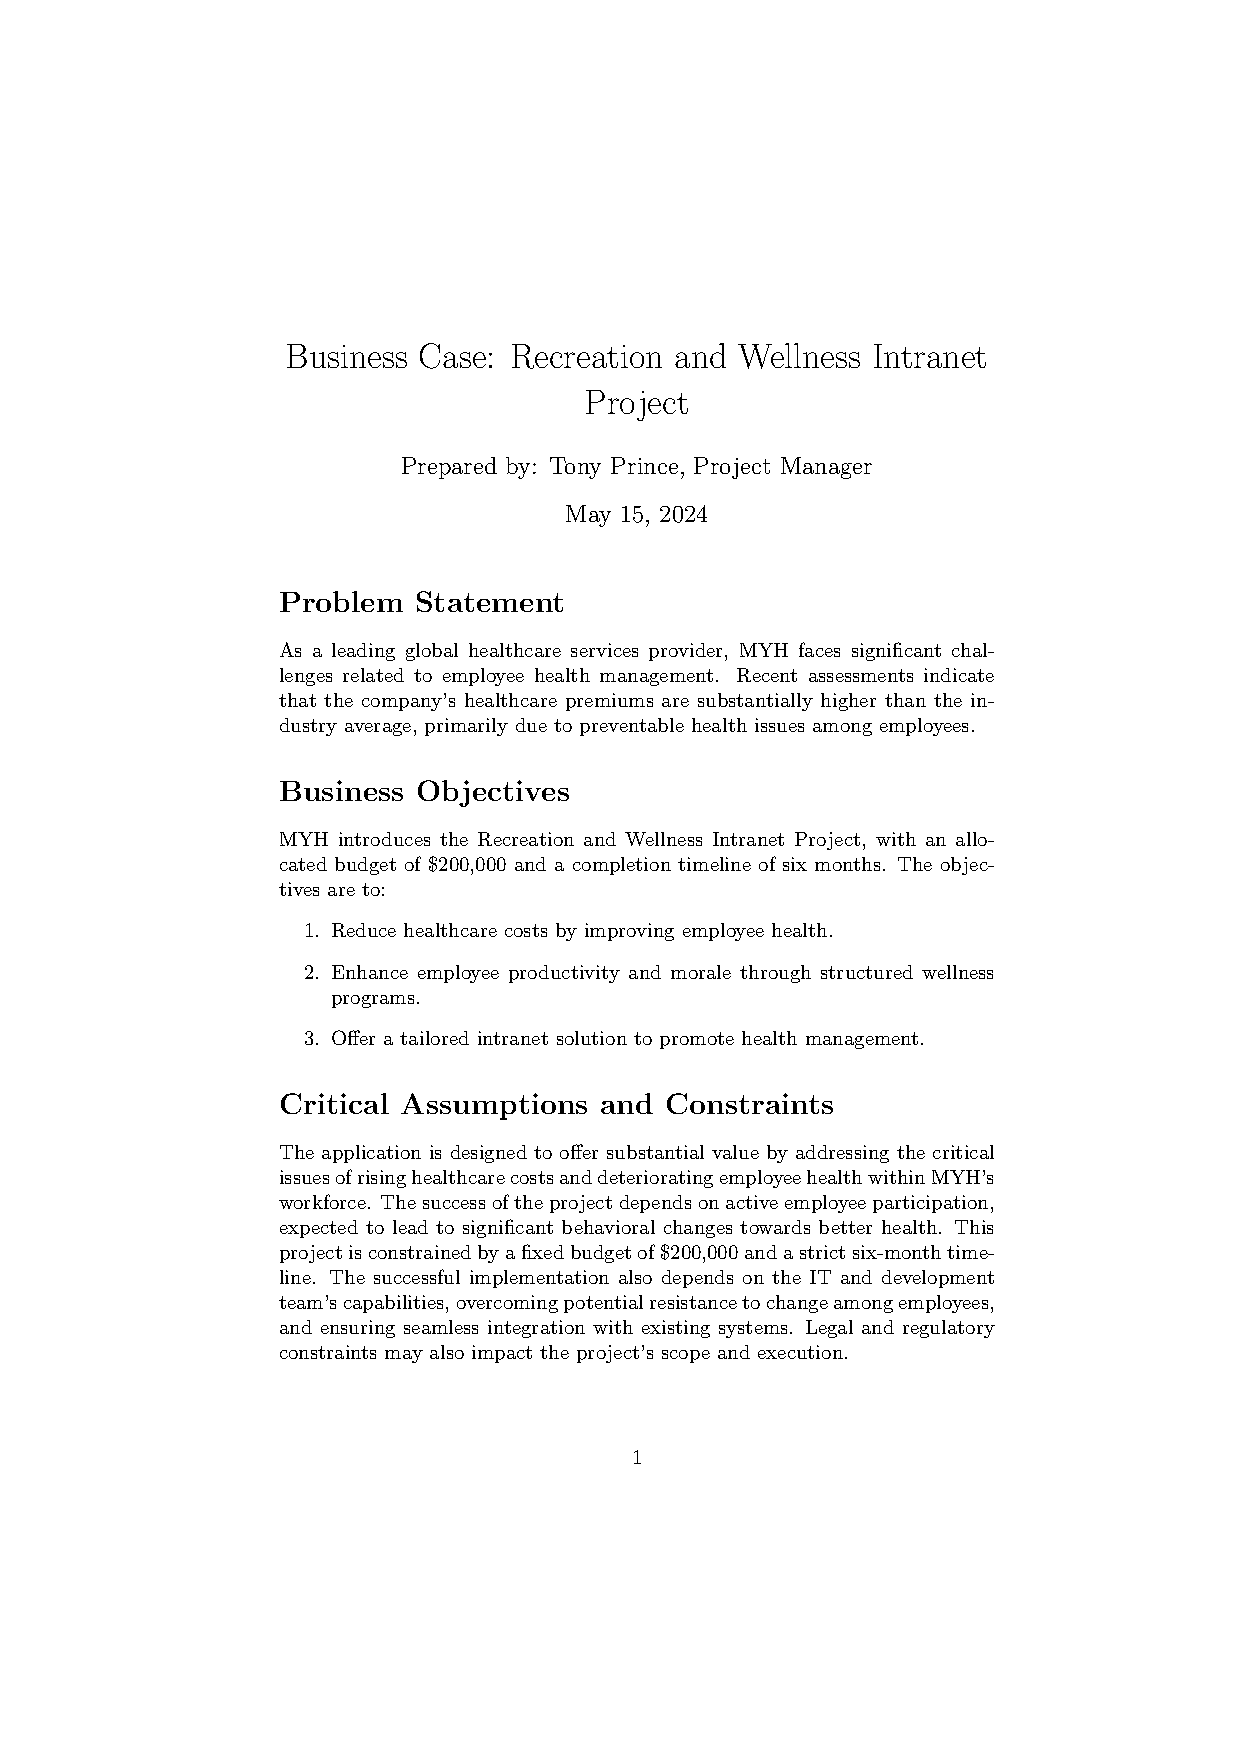
\includepdf[pages=-]{parts/part1/business_case.pdf}